% begin module cycloid-equations-ex7
\begin{frame}
\begin{example} %[Example 7, p. 660]
Find parametric equations of a cycloid made using a circle with radius $r$ that rolls along the $x$-axis such that $P$ hits the origin.
\begin{columns}[c]
\column{.4\textwidth}

\psset{xunit=1cm, yunit=1cm}
\begin{pspicture}(-1.000000, -5)(1.500000,5) 
\psframe*[linecolor=white](-1.000000,-5)(5.500000,5) 
\tiny 
\psaxesStandard{-0.500000}{-0.5}{3.2}{2.2}
%Calculator input: plotCurve{}(- \sin{}t+t, - \cos{}t+1, 0, \pi)
\parametricplot[linecolor=\psColorGraph, plotpoints=1000] { 0}{3.14159}{t t 57.29578 mul sin -1 mul add 1 t 57.29578 mul cos -1 mul add }

\psFullDot{2.094395102}{1}

%Function formula: - \sqrt{- (x-2/3 \pi+0.866025)^{2}+1}+1 
\psplot[linecolor=\psColorTangent, plotpoints=1000]{0.228380}{2.228360}{1 1 0.866025 3.14159 -0.666667 mul add x add 2 exp -1 mul add sqrt -1 mul add }
%Function formula: \sqrt{- (x-2/3 \pi+0.866025)^{2}+1}+1 
\psplot[linecolor=\psColorTangent, plotpoints=1000]{0.228380}{2.228360}{1 1 0.866025 3.14159 -0.666667 mul add x add 2 exp -1 mul add sqrt add }
\end{pspicture} 

\ \only<handout:0| -2>{%
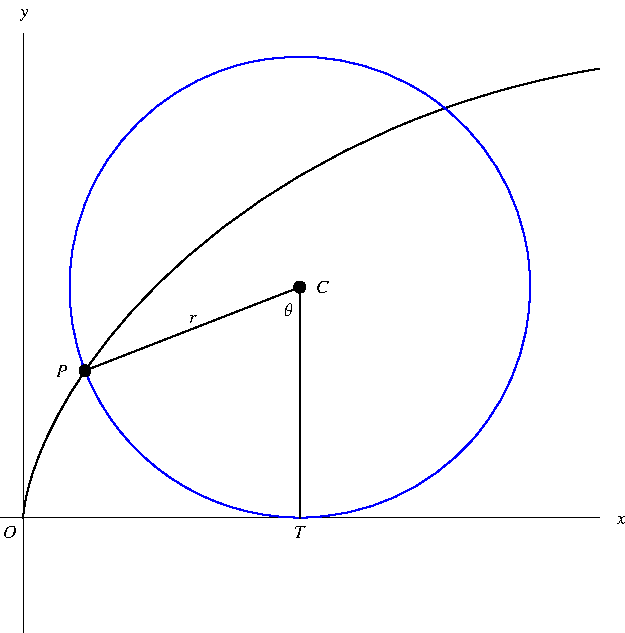
\includegraphics[width=5cm]{parametric-curves/pictures/11-01-cycloideqa.pdf}%
}%
\only<handout:0| 3>{%
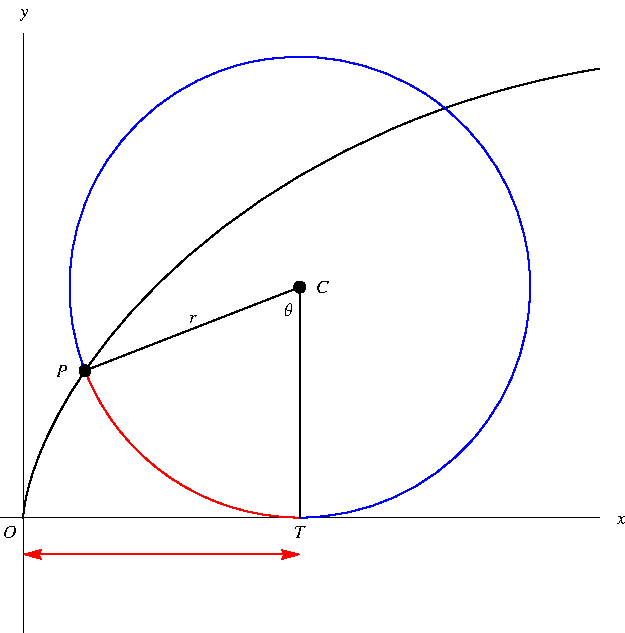
\includegraphics[width=5cm]{parametric-curves/pictures/11-01-cycloideqb.pdf}%
}%
\only<handout:0| 4>{%
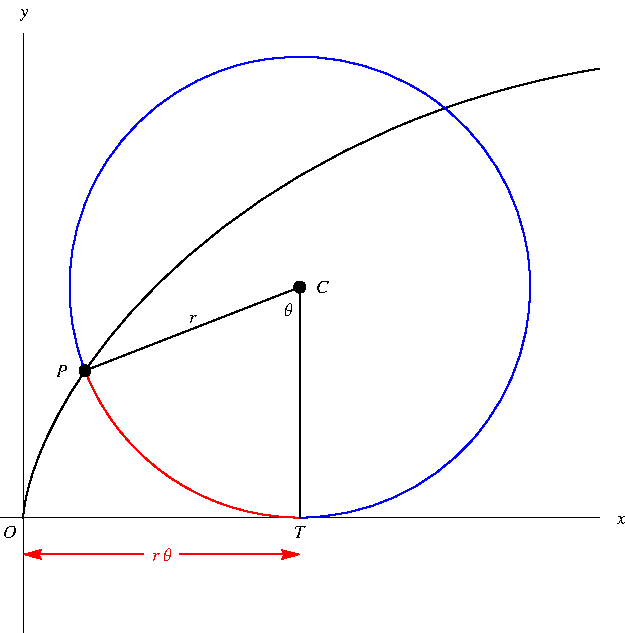
\includegraphics[width=5cm]{parametric-curves/pictures/11-01-cycloideqc.pdf}%
}%
\only<handout:0| 5>{%
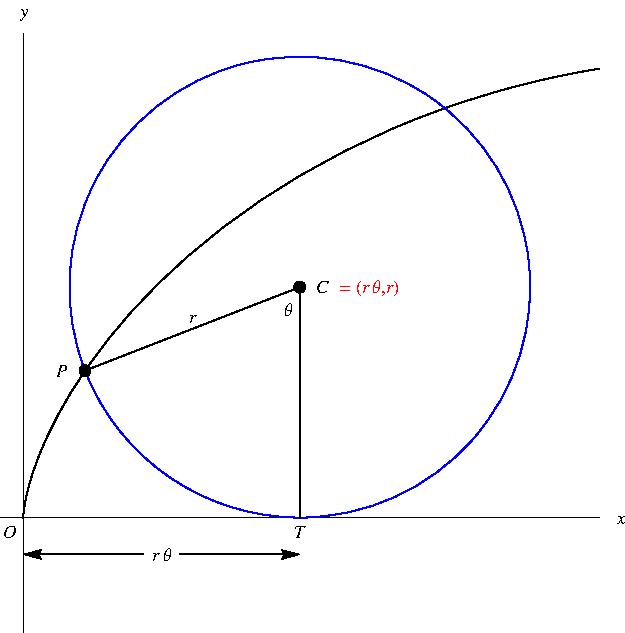
\includegraphics[width=5cm]{parametric-curves/pictures/11-01-cycloideqd.pdf}%
}%
\only<handout:0| 6>{%
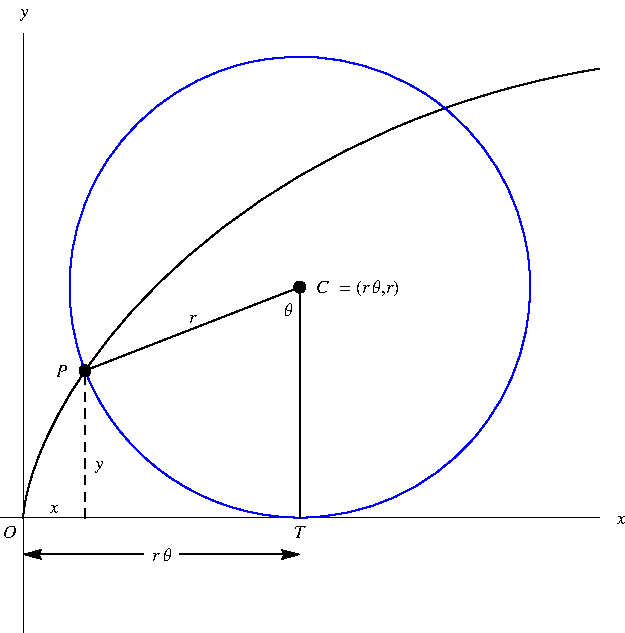
\includegraphics[width=5cm]{parametric-curves/pictures/11-01-cycloideqe.pdf}%
}%
\only<7->{%
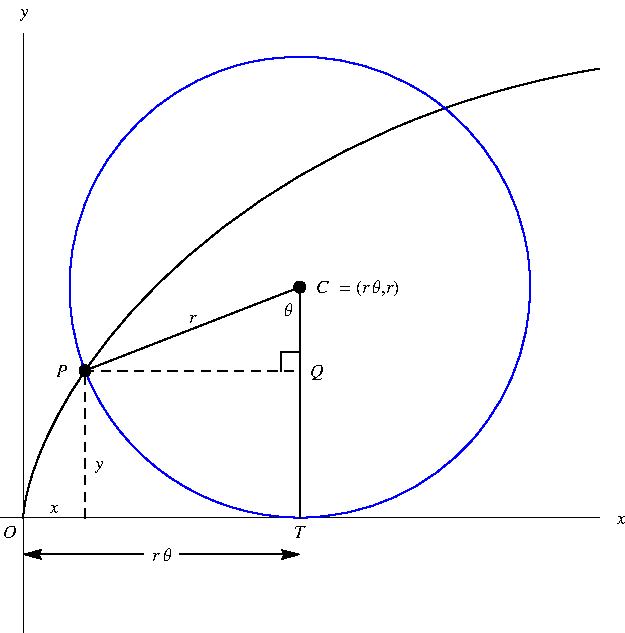
\includegraphics[width=5cm]{parametric-curves/pictures/11-01-cycloideqf.pdf}%
}%
\column{.6\textwidth}
\begin{itemize}
\item<2->  We choose our parameter to be $\theta$, the angle of rotation of the circle.
\item<3->  How far has the circle moved if it has rolled through $\theta$ radians?
\abovedisplayskip=0pt
\belowdisplayskip=0pt
\[
\uncover<3->{%
|OT| = \alert<handout:0| 4>{\textrm{arc} PT }%
}%
\uncover<4->{%
\alert<handout:0| 4>{ = r\theta}%
}%
\]
\item<5->  Then the center is $C = (r\theta , r)$.
\item<6->  Let the coordinates of $P$ be $(x,y)$.
\end{itemize}
\[
\begin{array}{cccccc}
\uncover<6->{%
\alert<handout:0| 8>{x}%
}&%
\uncover<6->{%
\alert<handout:0| 8>{=}%
}&%
\uncover<8->{%
\alert<handout:0| 8>{\alert<handout:0| 9-10>{|OT|} - \alert<handout:0| 11-12>{|PQ|}}%
}&%
\uncover<9->{%
=%
}&%
\uncover<10->{%
\alert<handout:0| 10>{r\theta}%
}%
\uncover<9->{-}%
\uncover<12->{%
\alert<handout:0| 12>{r\sin \theta}%
}\\%

\uncover<6->{%
\alert<handout:0| 13>{y}%
}&%
\uncover<6->{%
\alert<handout:0| 13>{=}%
}&%
\uncover<13->{%
\alert<handout:0| 13>{\alert<handout:0| 14-15>{|CT|} - \alert<handout:0| 16-17>{|CQ|}}%
}&%
\uncover<14->{%
=%
}&%
\uncover<15->{%
\alert<handout:0| 15>{r}%
}%
\uncover<14->{-}%
\uncover<17->{%
\alert<handout:0| 17>{r\cos \theta}%
}\\%
\end{array}
\]
\end{columns}
\uncover<18->{%
Therefore the equations are
\abovedisplayskip=0pt
\belowdisplayskip=0pt
\[
x = r(\theta - \sin \theta ),\qquad y = r(1-\cos \theta ),\qquad \theta \in \mathbb{R}
\]
}%
\end{example}
\end{frame}
% end module cycloid-equations-ex7
